\setcounter{chapter}{-1} % make this chapter 0
\chapter{Introduction}
%\addcontentsline{toc}{chapter}{Introduction} % but still display in TOC (see https://tex.stackexchange.com/a/222961)

Inspiration

\url{https://en.wikipedia.org/wiki/White_dwarf#Formation}

\url{https://en.wikipedia.org/wiki/Compact_star}

\section{The life and death of stars}

\begin{figure}
\centering
\usetikzlibrary{positioning}
\usetikzlibrary{shapes.symbols}
\usetikzlibrary{shadows}
\usetikzlibrary{trees}
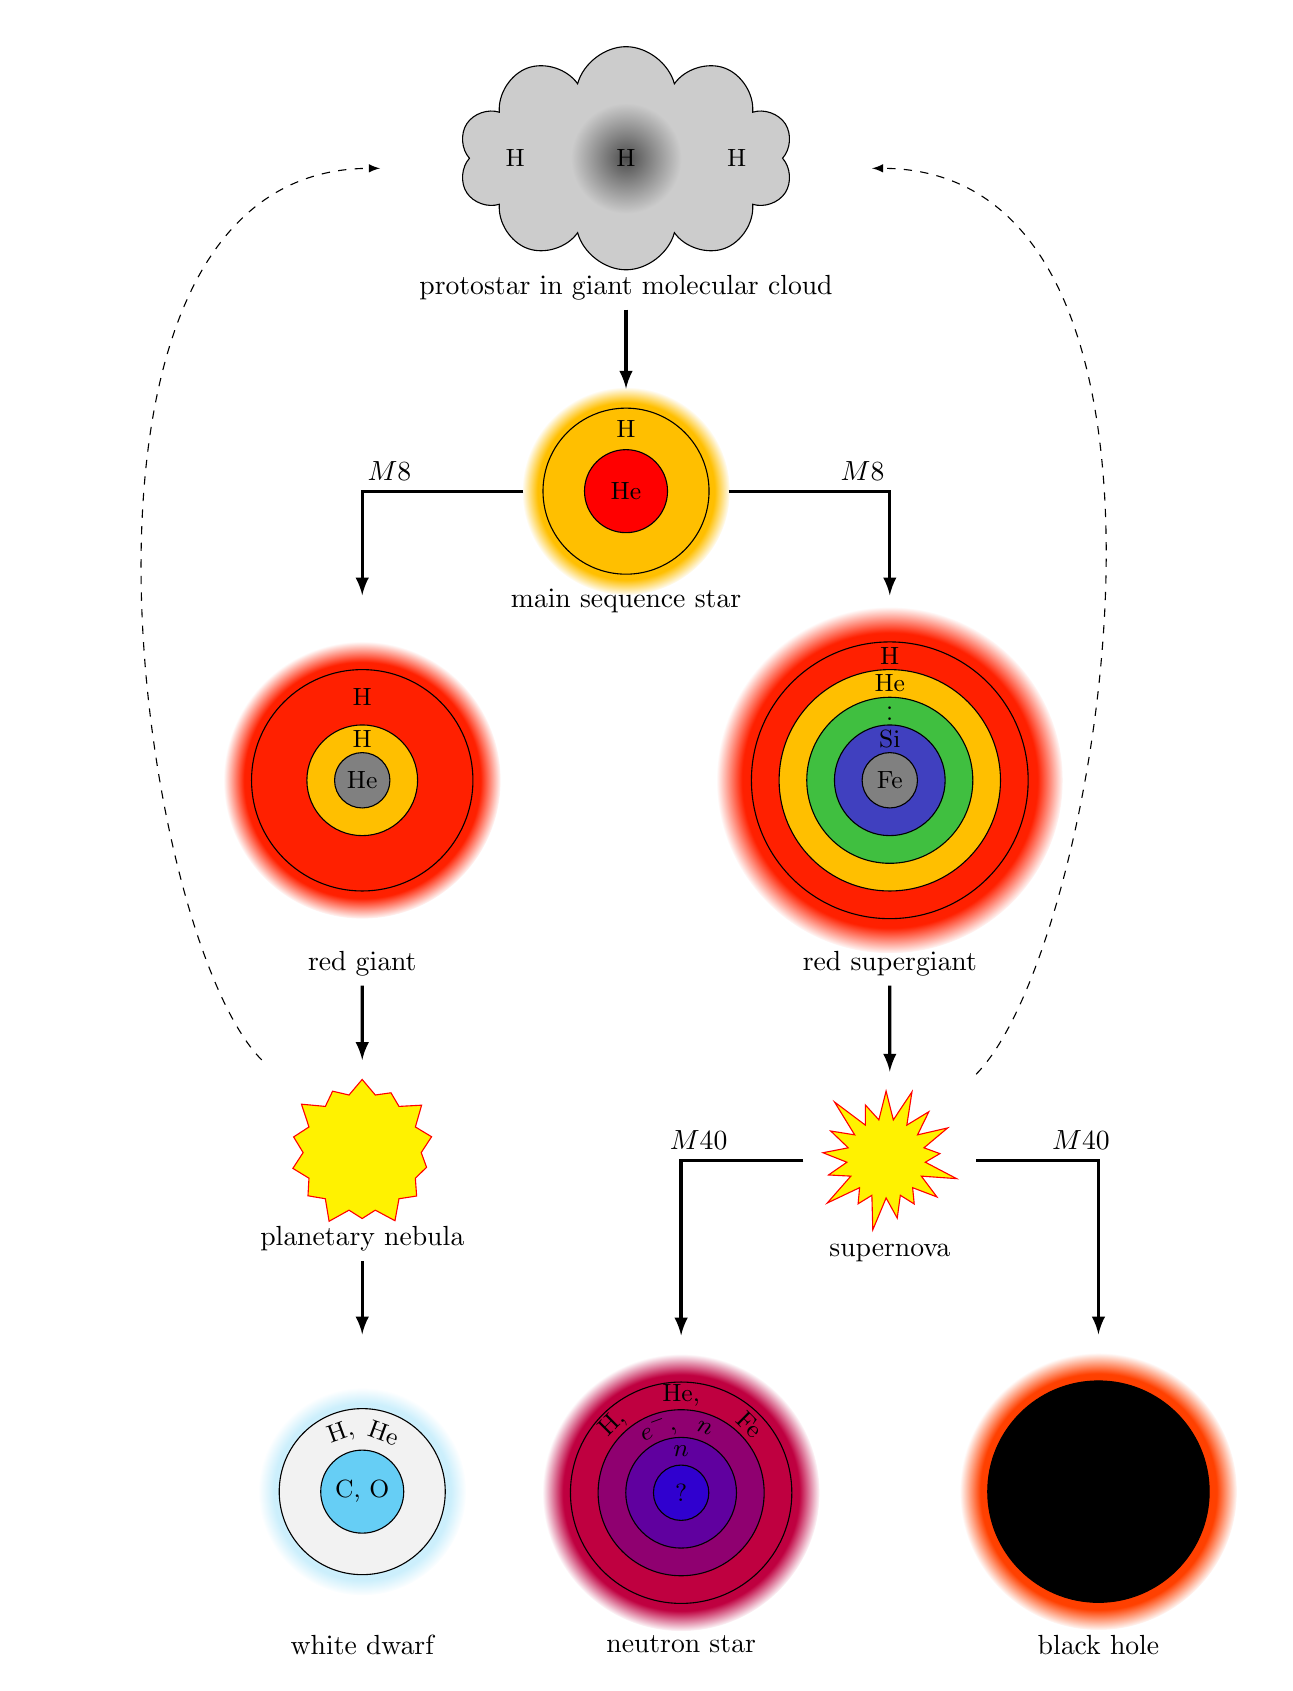
\begin{tikzpicture}[
	edge from parent/.style={draw,very thick,-latex},
	level distance=5cm,
	level 1/.style={level distance=4.1cm},
	level 2/.style={level distance=3.8cm, sibling distance=6.7cm},
	level 3/.style={level distance=4.7cm},
	level 4/.style={level distance=4.3cm, sibling distance=5.3cm},
	sibling distance=6cm,
	every label/.style={text width=4cm, text centered, inner sep=0pt, yshift=+2pt},
	element/.style={font=\small},
	dualpath/.style={
		edge from parent path={(\tikzparentnode\tikzparentanchor) -| (\tikzchildnode\tikzchildanchor)},
	},
	cloud/.pic={
		\node [draw, cloud, element, aspect=2, fill=gray, inner sep=10pt] {H};
	},
	protostar/.pic={
		\node [draw, cloud, aspect=2, fill=black!20!white, inner sep=20pt] {};
		\shade [even odd rule, inner color=black!70!white, outer color=black!20!white] circle (20pt);
		\node [element] at (0, 0) {H};
		\node [element] at (-40pt, 0) {H};
		\node [element] at (+40pt, 0) {H};
	},
	mainsequencestar/.pic={
		\draw[draw=black, fill=orange!50!yellow, circular glow={fill=orange!50!yellow}] circle [radius=30pt]; \node [element] at (90:22.5pt) {H};
		\draw[draw=black, fill=red] circle [radius=15pt]; \node [element] at (90:0pt) {He};
	},
	browndwarf/.pic={
		\filldraw[brown] circle [radius=20pt];
		\node [element] at (90:0pt) {H};
	},
	redgiant/.pic={
		\draw[draw=black, fill=red!75!orange, circular glow={fill=red!75!orange}] circle [radius=40pt]; \node [element] at (90:30pt) {H};
		\draw[draw=black, fill=orange!50!yellow] circle [radius=20pt]; \node [element] at (90:15pt) {H};
		\draw[draw=black, fill=gray] circle [radius=10pt]; \node [element] at (90: 0pt) {He};
		\draw[draw=none] (-60pt,-60pt) rectangle (+60pt,+60pt);
	},
	redsupergiant/.pic={
		\draw[draw=black, fill=red!75!orange, circular glow={fill=red!75!orange}] circle [radius=50pt]; \node [element] at (90:45pt) {H};
		\draw[draw=black, fill=orange!50!yellow] circle [radius=40pt]; \node [element] at (90:35pt) {He};
		\draw[draw=black, fill=green!50!gray] circle [radius=30pt]; \node [element] at (90:25pt) {$\vdots$ };
		\draw[draw=black, fill=blue!50!gray] circle [radius=20pt]; \node [element] at (90:15pt) {Si};
		\draw[draw=black, fill=gray] circle [radius=10pt]; \node [element] at (90:0pt) {Fe};
		\draw[draw=none] (-60pt,-60pt) rectangle (+60pt,+60pt);
	},
	supernova/.pic={
		\node[starburst, fill=yellow, draw=red, minimum size=2cm] {};
	},
	planetarynebula/.pic={
		\node[starburst, starburst points=14, starburst point height=0.25cm, fill=yellow, draw=red,  minimum size=2.0cm] {};
	},
	blackhole/.pic={
		\draw [fill=black, circular glow={fill=red!50!orange}] circle[radius=40pt];
		\draw[draw=none] (-50pt, -50pt) rectangle (+50pt, +50pt);
	},
	neutronstar/.pic={
		\draw[draw=black, fill=blue!  0!purple, circular glow={fill=blue!0!purple}] circle [radius=40pt]; \node [element, rotate=45] at (135:35pt) {H,}; \node [element] at ( 90:35pt) {He,}; \node [element, rotate=-45] at (45:35pt) {Fe};
		\draw[draw=black, fill=blue! 25!purple] circle [radius=30pt]; \node [element, rotate=+20] at (110:25pt) {$e^-$,}; \node [element, rotate=-20] at (70:25pt) {$n$};
		\draw[draw=black, fill=blue! 50!purple] circle [radius=20pt]; \node [element] at (90:15pt) {$n$};
		\draw[draw=black, fill=blue! 75!purple] circle [radius=10pt]; \node [element] at (90: 0pt) {?};
		\draw[draw=none] (-50pt, -50pt) rectangle (+50pt, +50pt);
	},
	whitedwarf/.pic={
		\draw[draw=black, fill=white! 90!gray, circular glow={fill=cyan! 20!white}] circle [radius=30pt]; \node [element, rotate=+20] at (110:22.5pt) {H,}; \node [element, rotate=-20] at (70:22.5pt) {He};
		\draw[draw=black, fill=cyan! 60!white] circle [radius=15pt]; \node [element] at (90:0pt) {C, O};
		\draw[draw=none] (-50pt, -50pt) rectangle (+50pt, +50pt);
	},
]

	\node (protostar) {\tikz \node [label={[text width=6.0cm]below:\subcaption{\label{fig:intro:star_evolution_protostar}protostar in giant molecular cloud}}] {\tikz \pic {protostar};};}
		child { node [label={[]below:\subcaption{\label{fig:intro:star_evolution_mainseq}main sequence star}}] {\tikz \node [] {\tikz \pic {mainsequencestar};};}
			child { node {\tikz \node [label={below:\subcaption{\label{fig:intro:star_evolution_red_giant}red giant}}] {\tikz \pic {redgiant};};}
				child { node (planetarynebula) {\tikz \node [label={below:\subcaption{\label{fig:intro:star_evolution_planetary_nebula}planetary nebula}}] {\tikz \pic {planetarynebula};};}
					child { node {\tikz \node [label={below:\subcaption{\label{fig:intro:star_evolution_white_dwarf}white dwarf}}] {\tikz \pic {whitedwarf};};} }
				} edge from parent [dualpath] node [above, anchor=south west, xshift=-2pt] {$M \lesssim 8 \solarmass$}
			}
			child { node {\tikz \node [label={below:\subcaption{\label{fig:intro:star_evolution_red_supergiant}red supergiant}}] {\tikz \pic {redsupergiant};};}
				child { node (supernova) [label={below:\subcaption{\label{fig:intro:star_evolution_supernova}supernova}}] {\tikz \node [] {\tikz \pic {supernova};};}
					child { node {\tikz \node [label={below:\subcaption{\label{fig:intro:star_evolution_neutron_star}neutron star}}] {\tikz \pic {neutronstar};};} edge from parent [dualpath] node[above, anchor=south west, xshift=-8pt] {$M \lesssim 40 \solarmass$} }
					child { node {\tikz \node [label={below:\subcaption{\label{fig:intro:star_evolution_black_hole}black hole}}] {\tikz \pic {blackhole};};} edge from parent [dualpath] node[above, anchor=south east, xshift=+8pt] {$M \gtrsim 40 \solarmass$} }
				}
				edge from parent [dualpath] node [above, anchor=south east, xshift=+2pt] {$M \gtrsim 8 \solarmass$}
			}
		};
	\draw [-latex, dashed] (supernova)       to [out= 45, in=  0, out looseness=0.5] (protostar);
	\draw [-latex, dashed] (planetarynebula) to [out=135, in=180, out looseness=0.5] (protostar);
\end{tikzpicture}
\caption{\label{fig:intro:star_evolution}%
	Simplified life cycle of stars and their main structure at every stage (not to scale).
}
\end{figure}

% planetary nebula -> releases ionized gas -> forms clouds
The mother of any star is an enormous accumulation of light elements like hydrogen called a \textbf{giant molecular cloud}, formed by the ashes of dying stars at the end of the life cycle we have just begun to describe.
Such clouds consist of matter weighing up to tens of millions solar masses, distributed with a relatively low average density over a huge area that up to hundreds of lightyears across.
Internally, the dynamics of a molecular cloud is chiefly governed by the attractive force of gravity between particles and the repulsive thermal pressure from their motion and collisions.

Due to the force of gravity, parts of the cloud can clump together in areas of greater density.
As more mass accumulates, the force of gravity attracting the surrounding material only increases, causing a snowball effect that only amplifies the growth of the clump.
Initially, the material is not so dense, and thermal radiation can escape outside, causing low temperatures and pressure and allowing the clump to contract with little resistance.
However, once the density becomes sufficiently high, thermal radiation can no longer find its way out and is trapped inside.
When this happens, the temperature increases, in turn increasing the outwards pressure that counteracts the inwards gravitational collapse and considerably slows down the contraction.
During this stage depicted in \cref{fig:intro:star_evolution_protostar}, as the child ``clump'' grows by sucking up material from its parent cloud, it receives the more honorable name \textbf{protostar}.

Sooner or later, the protostar has depleted the cloud of its available mass.
It then continues to contract, causing the temperature and pressure to increase, ultimately reaching a state of equilibrium with the gravitational collapse.
The protostar is then promoted to a \textbf{main sequence star}.
Provided that the protostar has accumulated at least $M \gtrsim 0.08 \solarmass$, the temperature will reach $T \gtrsim \SI{1e7}{\kelvin}$ -- sufficient for the fusion of hydrogen into helium to take place.
For billions of years, the star supports itself by burning hydrogen into helium.
The heavier helium is pulled into the central regions of the star, establishing a helium \emph{core} surrounded by an \emph{envelope} constisting of the lighter hydrogen, as shown in \cref{fig:intro:star_evolution_mainseq}.

What happens after most of the hydrogen has burnt up depends heavily on the mass of the star.
Stars up to $M \lesssim 8 \solarmass$ evolve into \textbf{red giants}.
As the hydrogen fails to support the star, the core begins to contract again.
For heavier red giants, the temperature can increase to $T \gtrsim \SI{1e8}{\kelvin}$, activating both fusion of helium to carbon and carbon to oxygen, but the temperature is too low for fusion of heavier elements.
The core develops shells with elements of increasing weight towards the center as shown in \cref{fig:intro:star_evolution_red_giant}, from hydrogen to helium, carbon, or oxygen, depending on the exact mass of the star.
Due to the sudden increase in temperature, much energy is transported into the envelope, where it ignites leftover hydrogen and inflates the envelope up to 200 solar radii -- hence the name of the star.

Eventually, explosions in the envelope of a red giant trigger unstable pulsations of the hydrogen envelope.
This causes a \textbf{planetary nebula}, depicted in \cref{fig:intro:star_evolution_planetary_nebula} -- an ejection of the outer shells of the red giant into new interstellar clouds from which new starts can be born at a restart of the cycle.
The remaining inert core that is intact from the nebula forms a \textbf{white dwarf}.
Illustrated in \cref{fig:intro:star_evolution_white_dwarf}, a white dwarf is essentially the core of the preceeding red giant that is intact after the planetary nebula.
Since no further reactions occur, it is supported against collapse solely by electron degeneracy pressure.
White dwarves can be as hot as $T \approx \SI{1e7}{\kelvin}$ upon formation, but gradually cool down as they radiate away their energy.
Importantly, white dwarves can only support themselves for masses up to the Chandrasekhar limit $M \lesssim 1.4 \solarmass$.
\TODO{cooling etc}

If the mass of a main sequence star exceeds $M \gtrsim 8 \solarmass$, it essentially becomes a more dramatic a red giant -- namely a \textbf{red supergiant}.
The increased mass sends the temperature soaring well above $T \gtrsim \SI{1e8}{\kelvin}$, activating not only fusion from hydrogen to helium, carbon and oxygen, but even fusion to heavier elements such as neon and iron.
When the reactions reach iron, something dramatic happens.
In contrast to elements lighter than iron, fusion from iron or heavier elements \emph{require} energy instead of releasing it.
The burning therefore stops at iron.
At this point, the core of a red supergiant is so massive due to the more massive elements that it exceeds the Chandrasekhar limit.
Thus, the core collapses in an explosion called a \textbf{supernova}, illustrated in \cref{fig:intro:star_evolution_supernova}.
\TODO{iron peak graph?}

For supergiants whose mass does not exceed $M \lesssim 40 \solarmass$, the core left behind by the supernova is called a \textbf{neutron star}.
The core collapse of the supergiant has compressed the core past the white dwarf stage, reaching a new equilibrium composition of neutrons, protons, hyperons, leptons and possibly quarks.
Like white dwarves, neutron stars are ovens that are burnt out, and only continue to cool down and shine.
\TODO{temperature? new 1e11-1e12 K, quickly decays to 1e6, then radiate away and cool down}

Even more massive supergiants with more than $M \gtrsim 40 \solarmass$ experience such a tremendous force of gravity that they collapse directly to \textbf{black holes}, depicted in \cref{fig:intro:star_evolution_black_hole}.

\section{From proposition to observation and theory of neutron stars}


Since the dawn of mankind, humans have gazed upon the night sky with great curiosity of what lies out in the universe.
\begin{itemize}
\item Establish the importance of studying stars from an existential point of view.
\item Give a brief historical review of how our view of stars and the universe has changed, from the nonscientific views of the earliest days to the scientific viewpoint of the modern age.
\end{itemize}

After the discovery of the neutron in 1933, scientists soon proposed the existence of stars consisting of neutrons.
\begin{itemize}
\item Explain why neutron stars are plausible, from the original ``ignorant'' point of view before one has a good theoretical understanding of neutron stars.
\item Review the hypotheses that came from the initial theoretical work on neutron stars, before any observation was made.
\end{itemize}

In 1967, Jocelyn Bell and Antony Hewish discovered the first known neutron star.
\begin{itemize}
\item Review observations that have been made from neutron stars up until today.
\item Connect the observations made to the theoretical hypotheses from the last paragraph.
\end{itemize}

Today, scientists have a good understanding of neutron stars.
\begin{itemize}
\item Explain the modern, ``perfect'' understanding of neutron stars, that have not been covered by the ``naive'' view in the last two paragraphs.
\item Explain that neutron stars are formed by supernova explosions.
\item Explain that neutron stars are the smallest and densest class of stars that have been observed.
\item Explain that neutron stars are kept stable by the balance between gravitational attraction and Pauli pressure.
\end{itemize}

Being one of the most exotic types of objects humanity has observed, neutron stars are a gateway to developing our understanding of new, hypothetical astronomical objects.
\begin{itemize}
\item Explain why it is important to understand neutron stars first (even if others already understand them), in order to do new and interesting work.
\item Explain the possibility that neutron stars can develop into even more, currently hypothetical classes of stars, such as quark stars.
\end{itemize}

\section{Outline of this thesis}

In this thesis, we develop the theoretical tools necessary to study stars made of free neutrons, calculate their mass-radius curve and study their stability.
\begin{itemize}
\item State the content of this thesis, distinguishing between the theoretical tools we develop, and the results that we obtain by calculations with these tools.
\item Although these are not new findings but rather a review, this is our ``niche''.
\item To ``occupy our niche'', this paragraph should explain \emph{why} this particular content is the most natural buildup for a thesis on neutron stars.
\end{itemize}

In \textbf{\cref{chap:tov}}, we derive the \textbf{Tolman-Oppenheimer-Volkoff system of equations}
\begin{align*}
	\odv{P}{r} &= -\frac{G m \epsilon}{r^2 c^2} \left( 1 + \frac{P}{\epsilon} \right) \left( 1 + \frac{4 \pi r^3 P}{m c^2} \right) \left( 1 - \frac{2 G m}{r c^2} \right)^{-1} , \\
	\odv{m}{r} &= \frac{4 \pi r^2 \epsilon}{c^2} ,
\end{align*}
from the theory of general relativity.
\begin{itemize}
\item Explain why Newtonian gravity does not suffice to study stars, and that the relativistic effects of Einstein's theory is needed.
\item Explain the importance of the TOV equations for the study of \emph{any} kind of star.
\item Explain that the three unknowns in the equation are the pressure $P$, mass $m$ and energy density $\epsilon$.
      Since there are only two equations, we must find an additional one to solve for the unknowns.
      This is the equation of state $\epsilon = \epsilon(P)$, which is outside the scope of general relativity and must be found by statistical physics and quantum theory.
\end{itemize}

In \textbf{\cref{chap:tft}}, we will study \textbf{thermal field theory} -- the formalism needed to find the effects of quantum fields at nonzero temperature.
\begin{itemize}
\item Explain that thermal field theory is the ``missing link'' needed to find $\epsilon$ in the Tolman-Oppenheimer-Volkoff equation.
\item Present the buildup of this chapter: the partition function is needed for finding expectation values of thermodynamic variables, the partition function can be found by a path integral.
\item We first show how one does the path integral for bosons with complex numbers, then introduce anticommuting Grassmann numbers to find the path integral for fermions.
\end{itemize}

In \textbf{\cref{chap:nstars}}, we finally put together the pieces of \cref{chap:tov} and \cref{chap:tft} and study \textbf{neutron stars}.
\begin{itemize}
\item Make very clear that while chapter 1 and 2 ``only'' develop theoretical tools, chapter 1+2=3 puts the tools to work together and constitutes our ``results'' chapter.
\item Having found the partition function for free fermions in \cref{chap:tft}, we find the equation of state $\epsilon = \epsilon(P)$ for a gas of free neutrons.
\item Then we insert the equation of state into the Tolman-Oppenheimer-Volkoff equations and solve them, which yield the mass-radius-curve of neutron stars parametrized by their central pressure.
\item This is our ``results'', then we compare them to observations and earlier theoretical work.
\item Finally, we study the stability of the stars we have found.
\end{itemize}

In \textbf{\cref{chap:gr}}, we give a comprehensive \textbf{review of the theory of general relativity}.
\begin{itemize}
\item Say that this appendix enables readers unfamiliar with general relativity to understand all aspects of it that are needed for our purposes.
\end{itemize}

In \textbf{\cref{chap:relfluid}}, we study \textbf{relativistic fluid mechanics}.
\begin{itemize}
\item Assuming familiarity with general relativity, we derive all results needed to study the stability of stars.
\end{itemize}

In \textbf{\cref{chap:matsum}}, we describe the technique of \textbf{Matsubara frequency summation}.
\begin{itemize}
\item This is an elegant mathematical tool that is extremely useful to perform calculations in thermal field theory.
\item Say that this summation on its own is purely mathematical, and that the results thereof can be considered as mathematical identities only, when they are applied in the chapter on thermal field theory.
\item However, note that the results of the mathematical identities are of great physical interest, as it is precisely these identities that give rise to the bosonic and fermionic distributions.
\end{itemize}

In \textbf{\cref{chap:integrals}}, we list all integrals used throughout this thesis with pure proofs.

In \textbf{\cref{chap:code}}, we list all source code used for numerical work in this thesis.
